% A simple cycle
% Author : Jerome Tremblay
\documentclass{standalone}
\usepackage{tikz}
\begin{document}
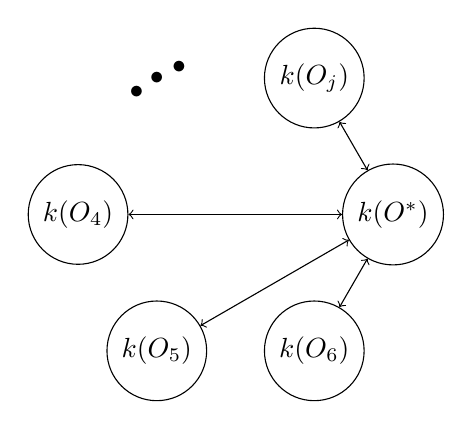
\begin{tikzpicture}

\def \n {6}
\def \radius {2cm}
\def \margin {4} % margin in angles, depends on the radius

    \node[draw, circle] (o) at ({360/\n*(0)}:2cm) {$k(O^*)$};
\foreach \s in {4,...,\n}
{
    \node[draw, circle]  (v) at ({360/\n * (\s - 1)}:\radius) {$k(O_\s)$};
  %\draw[->, >=latex] ({360/\n * (\s - 1)+\margin}:\radius) 
  %  arc ({360/\n * (\s - 1)+\margin}:{360/\n * (\s)-\margin}:\radius);
    \draw[<->] (o) edge (v);
}
    \node[draw, circle] (v) at ({360/\n*(1)}:\radius) {$k(O_j)$};
\draw[<->] (o) edge (v);

\node at ({360/\n*(2)}:\radius) {$\bullet$};
\node at ({360/\n*(2.15)}:\radius) {$\bullet$};
\node at ({360/\n*(1.85)}:\radius) {$\bullet$};
\end{tikzpicture}
\end{document}

